\section{Fundamentação Teórica}
\subsection{Modelos de cores}

\begin{frame}{Introdução}
\begin{itemize}
    \item Os seres humanos têm a capacidade de discernir milhares de tonalidades e intensidades
    \item A percepção humana das cores se dá pela ativação de células nervosas que enviam mensagens ao cérebro sobre brilho (\textit{brightness}), matiz (\textit{hue}) e saturação (\textit{saturation})
    \item As cores podem ser especificadas por modelos matemáticos em tuplas de números em um sistema de coordenadas
\end{itemize}
\end{frame}

%------------------------------------------------------
\begin{frame}{Diagrama de cromaticidade CIE 1931}
\begin{columns}
\column{0.5\textwidth}
\begin{itemize}
    \item Primeiro modelo matemático de especificação numérica da cor
    \item Componente de luminância Y; X e Z de cromaticidade (tristímulus)
    \item Derivações do CIE XYZ: \textbf{CIE 1976 $L^*u^*v^*$} e \textbf{1976 CIE $L^*a^*b^*$}
\end{itemize}
\column{0.5\textwidth}
\begin{figure}[!h]
  \centering
  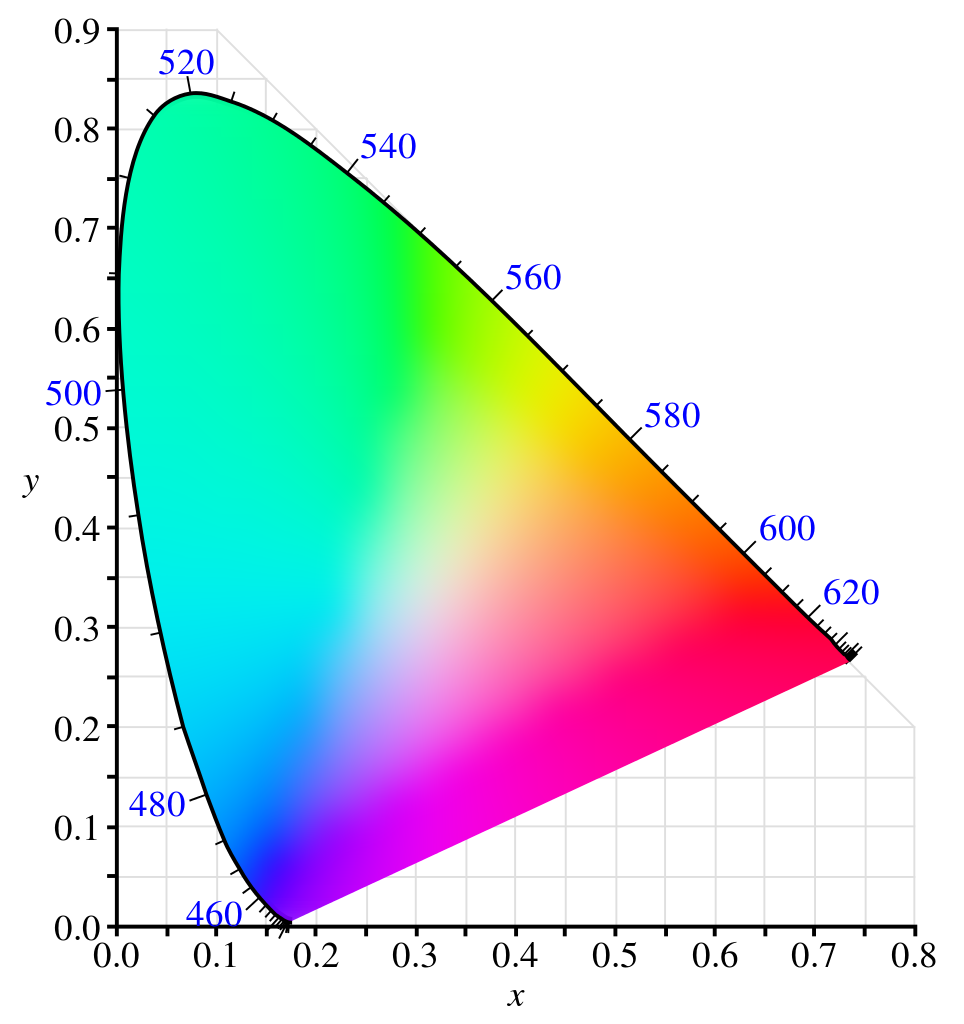
\includegraphics[width=1\textwidth]{cie-cromaticity-diagram}
\end{figure}
\end{columns}
\end{frame}

%------------------------------------------------------
\begin{frame}{Modelo RGB}
\begin{columns}
\column{0.5\textwidth}
\begin{itemize}
    \item Modelo de cores aditivo
    \item Baseado na teoria tricromática de Thomas Young e Hermann Helmholtz em meados do século 19
\end{itemize}
\column{0.5\textwidth}
\begin{figure}[!h]
  \centering
  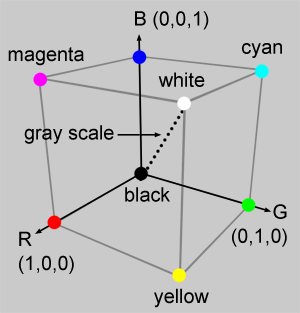
\includegraphics[width=.9\textwidth]{rgb-cube}
\end{figure}
\end{columns}
\end{frame}

%------------------------------------------------------
\begin{frame}{Modelos da família YUV}
\begin{itemize}
    \item Y = luminância, U = Azul - Y, V = Vermelho - Y
    \item Utilizado em sistemas de transmissão analógica de televisão nos padrões PAL e SECAM
    \item YCbCr é um modelo desta família e é largamente utilizado em vídeos digitais
\end{itemize}
\begin{equation*}
  \begin{bmatrix}
    Y \\ Cb \\ Cr
  \end{bmatrix} = 
  \begin{bmatrix}
     0.299 &  0.587 &  0.114 \\
    -0.169 & -0.331 &  0.5   \\
     0.5   & -0.419 & -0.081 \\
  \end{bmatrix}
  \begin{bmatrix}
    R \\ G \\ B
  \end{bmatrix}
\end{equation*}
\end{frame}

%------------------------------------------------------
\begin{frame}{Modelos da família HSI}
\begin{itemize}
    \item  (I)ntensidade é decomposta da informação de crominância
\end{itemize}
\begin{align*}
\begin{split}
  H &=  \begin{cases}
            60\ffrac{(G - B)}{M - m}, & \text{se}\ M = R\\[0.7em]
            60\ffrac{(B - R)}{M - m} + 120, & \text{se}\ M = G\\[0.7em]
            60\ffrac{(R - G)}{M - m} + 240, & \text{se}\ M = B
       \end{cases}
  \\[0.5em]
  S &=  \begin{cases}
            \ffrac{(M - m)}{M}, \quad &\text{se}\ M \neq 0\\[0.7em]
            0, \quad &\text{caso contrário}\\
       \end{cases}
  \\[0.5em]
  V &= M
\end{split}
\end{align*}
\end{frame}

%------------------------------------------------------
\subsection{Teoria fuzzy}
\begin{frame}{Introdução}
\begin{itemize}
    \item Visão tradicional e alternativa da ciência sobre a incerteza \citep{klir:95}
    \item Com base na ideia moderna de que a incerteza é algo útil na ciência, Zadeh propôs a teoria de conjuntos \emph{fuzzy}
    \item Capacidade de conjuntos \emph{fuzzy} expressarem transições graduais de pertinência e não pertinência
    \item Representação significativa e poderosa da medida de incerteza
    \item Forma de expressar conceitos vagos em linguagem natural
\end{itemize}
\end{frame}

%------------------------------------------------------
\begin{frame}{Conjuntos \emph{fuzzy}}
Da teoria de conjuntos clássicos tem-se a função característica:
\begin{equation*}
  \mu_A(x) =  \begin{cases}
                1 \quad \text{se}\ x \in A \\
                0 \quad \text{se}\ x \notin A
              \end{cases}
\end{equation*}

Que é um mapeamento dos elementos de $U$ no conjunto binário $\{0, 1\}$:
\begin{equation*}
  \mu_A =  U \rightarrow \{0, 1\}
\end{equation*}


Em conjuntos \emph{fuzzy}, generalização aplicada no intervalo $[0, 1]$:
\begin{equation*}
  \mu_A =  U \rightarrow [0, 1]
\end{equation*}
\end{frame}

%------------------------------------------------------
\begin{frame}{Conjuntos \emph{fuzzy}}

\begin{block}{Definição de conjuntos \emph{fuzzy}}
Um conjunto \emph{fuzzy} $A$ é um subconjunto do conjunto universo $U$ formado por pares ordenados de um elemento qualquer $x$ e seu grau de pertinência dado por $\mu_A(x)$, da forma:

\begin{equation*}
  A =  \{(x, \mu_A(x)) \ |\ x \in U\}
\end{equation*}
\end{block}

As noções de inclusão, união, intersecção, complemento, relação, convexidade, etc., oriundas da teoria de conjuntos clássica, são estendidas a esses conjuntos \citep{zadeh:65}.

\end{frame}

%------------------------------------------------------
\begin{frame}{Representação gráfica das principais propriedades dos conjuntos \emph{fuzzy}}
\begin{figure}[!h]
  \centering
  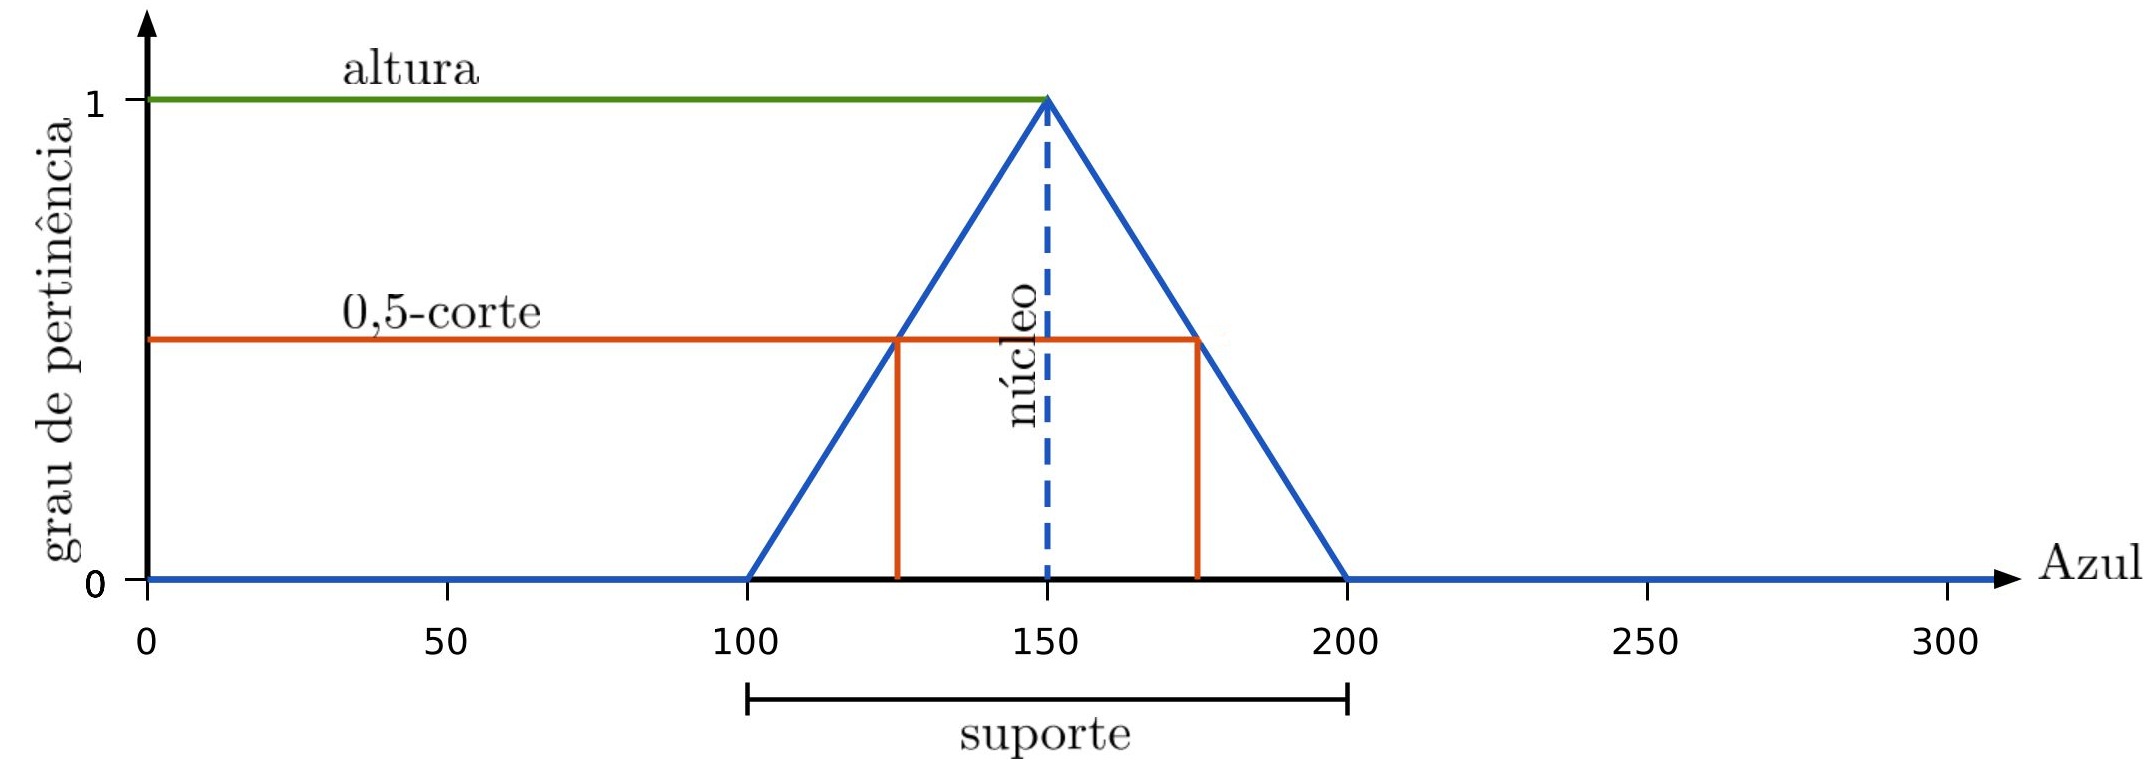
\includegraphics[width=1\textwidth]{fuzzy_definitions}
\end{figure}
\end{frame}

%------------------------------------------------------
\begin{frame}{Números \emph{fuzzy}}
Um número \emph{fuzzy} é um tipo especial de conjunto \emph{fuzzy} definido no conjunto $\mathbb{R}$ dos números reais, da forma \citep{klir:95}:
\begin{equation*}
  A : \mathbb{R} \rightarrow [0, 1]
\end{equation*}

Para que $A$ seja, de fato, um número \emph{fuzzy}, o conjunto universo no qual $\mu_A$ está definida deve ser $\mathbb{R}$ e as seguintes propriedades devem ser satisfeitas \citep{barros:06}:

\hspace{4pt}(i) todos os $\alpha$\emph{-corte} de $A$ são não vazios, com $0 \leq \alpha \leq 1$\\
\hspace{2pt}(ii) todos os $\alpha$\emph{-corte} são intervalos fechados de $\mathbb{R}$\\
(iii) $suporte(A) = \{x \in U \ |\ \mu_A(x) > 0\}$

\end{frame}

%------------------------------------------------------
\begin{frame}{Funções de pertinência}
Um número \emph{fuzzy} $A$ é dito triangular se sua função de pertinência, denotada por $\mu_{A}(x)$, é da forma:

\begin{columns}
\column{0.5\textwidth}
\begin{equation*}
  \mu_A(x) =  \begin{cases}
                \ffrac{x - a}{m - a}, &\text{se}\ a < x \leq m\\[0.5em]
                \ffrac{b - x}{b - m}, &\text{se}\ m < x < b\\[0.5em]
                0, &\text{c.c.}
              \end{cases}
\end{equation*}

\column{0.5\textwidth}
\begin{figure}[!h]
  \centering
  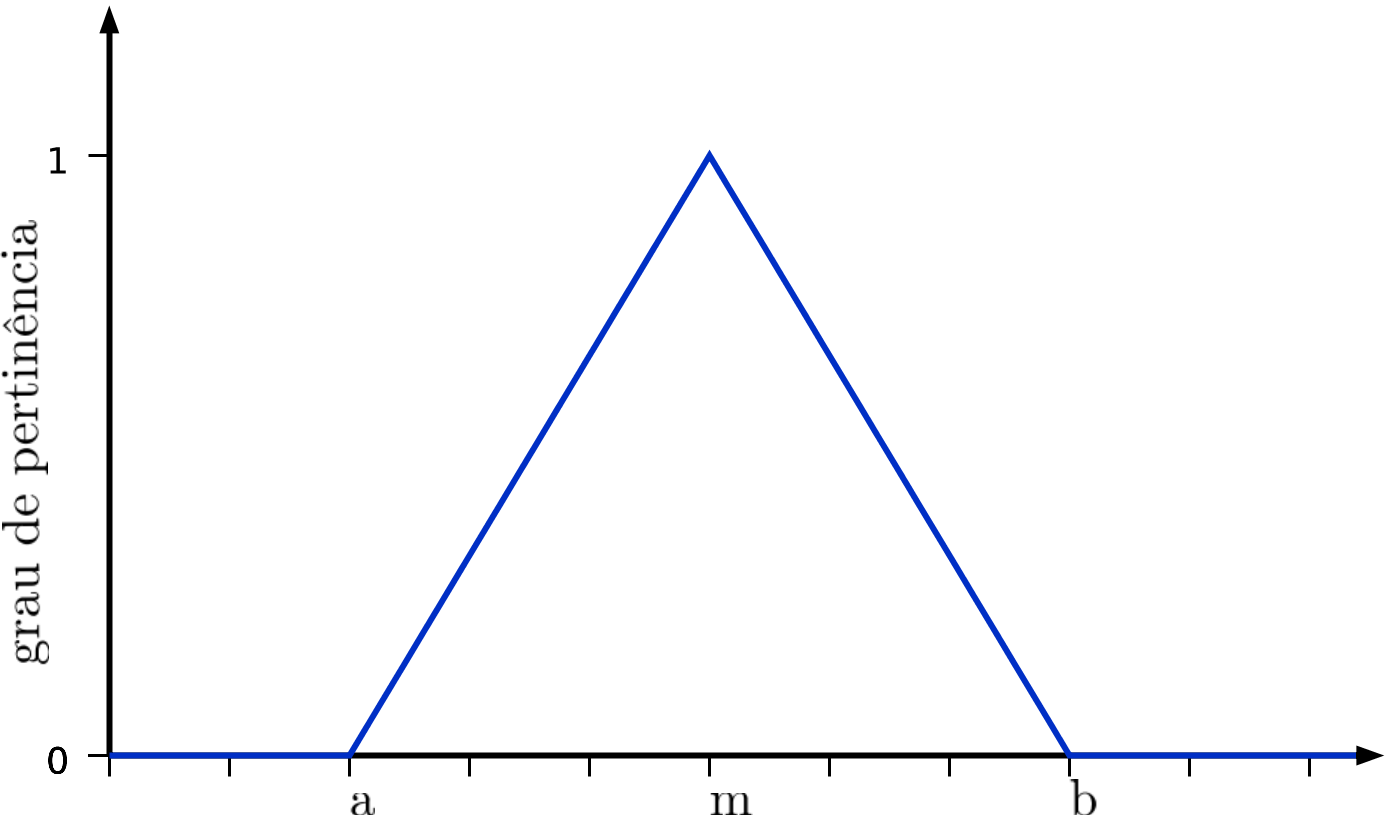
\includegraphics[width=1\textwidth]{funcao_triangular}
\end{figure}
\end{columns}
\end{frame}

%------------------------------------------------------
\begin{frame}{Funções de pertinência}
Um número \emph{fuzzy} $A$ é dito trapezoidal se sua função de pertinência, denotada por $\mu_{A}(x)$, é da forma:

\begin{columns}
\column{0.5\textwidth}
\begin{equation*}
  \mu_A(x) =  \begin{cases}
                \ffrac{x - a}{b - a}, & \text{se}\ a < x < b\\[0.5em]
                1, & \text{se}\ b \leq x \leq c\\[0.5em]
                \ffrac{d - x}{d - c}, & \text{se}\ c < x < d\\[0.5em]
                0, & \text{c.c.}
              \end{cases}
\end{equation*}

\column{0.5\textwidth}
\begin{figure}[!h]
  \centering
  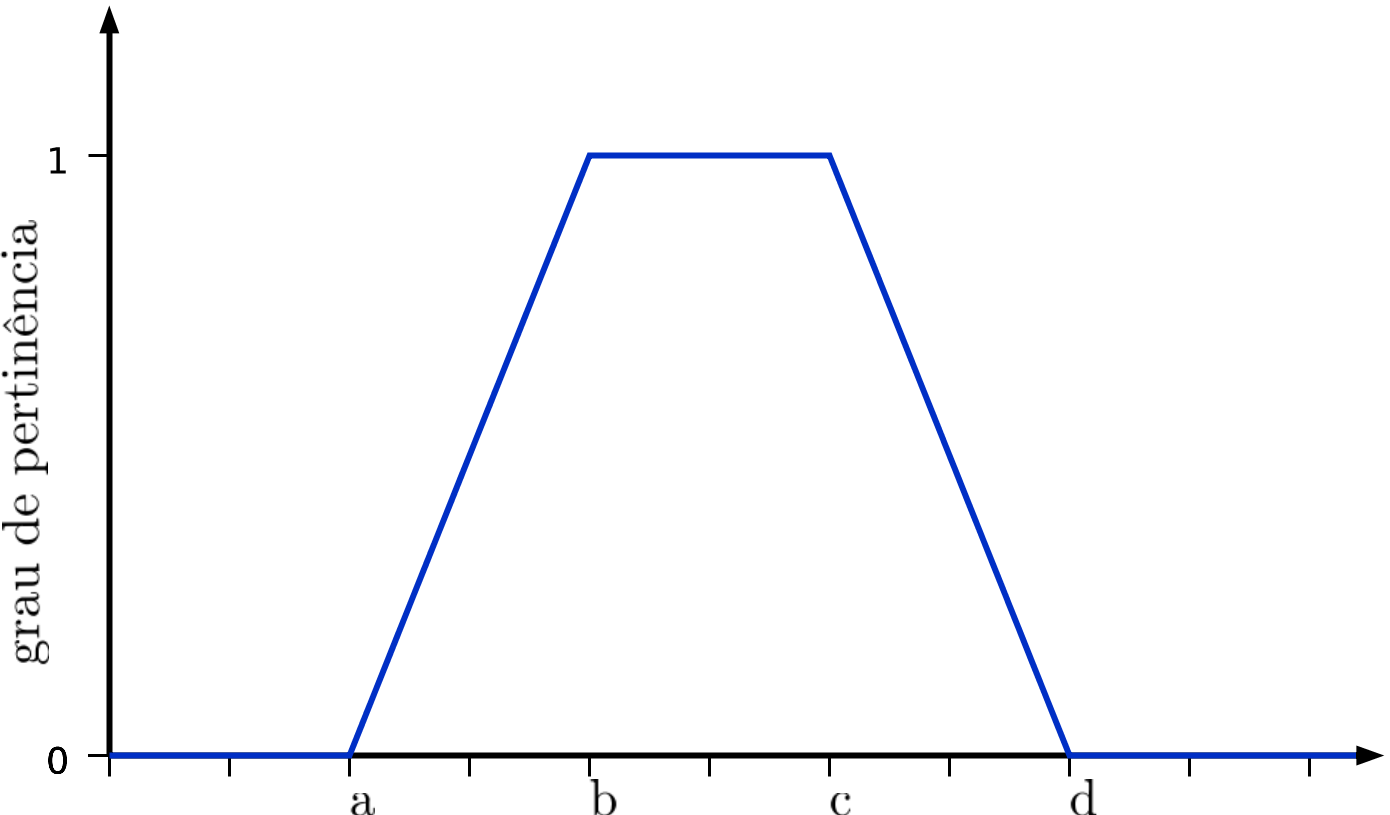
\includegraphics[width=1\textwidth]{funcao_trapezoidal}
\end{figure}
\end{columns}
\end{frame}

%------------------------------------------------------
\begin{frame}{Funções de pertinência}
Um número \emph{fuzzy} $A$ é dito gaussiano se sua função de pertinência, denotada por $\mu_{A}(x)$, é da forma:

\begin{columns}
\column{0.5\textwidth}
\begin{equation*}
  \mu_A(x) =  \begin{cases}
                \exp{\big(-\ffrac{{(x - m)}^2}{\sigma} \big)}, \\ \text{se}\ m - \sigma \leq x \leq m + \sigma\\[0.5em]
                0, \ \text{c.c.}
              \end{cases}
\end{equation*}

\column{0.5\textwidth}
\begin{figure}[!h]
  \centering
  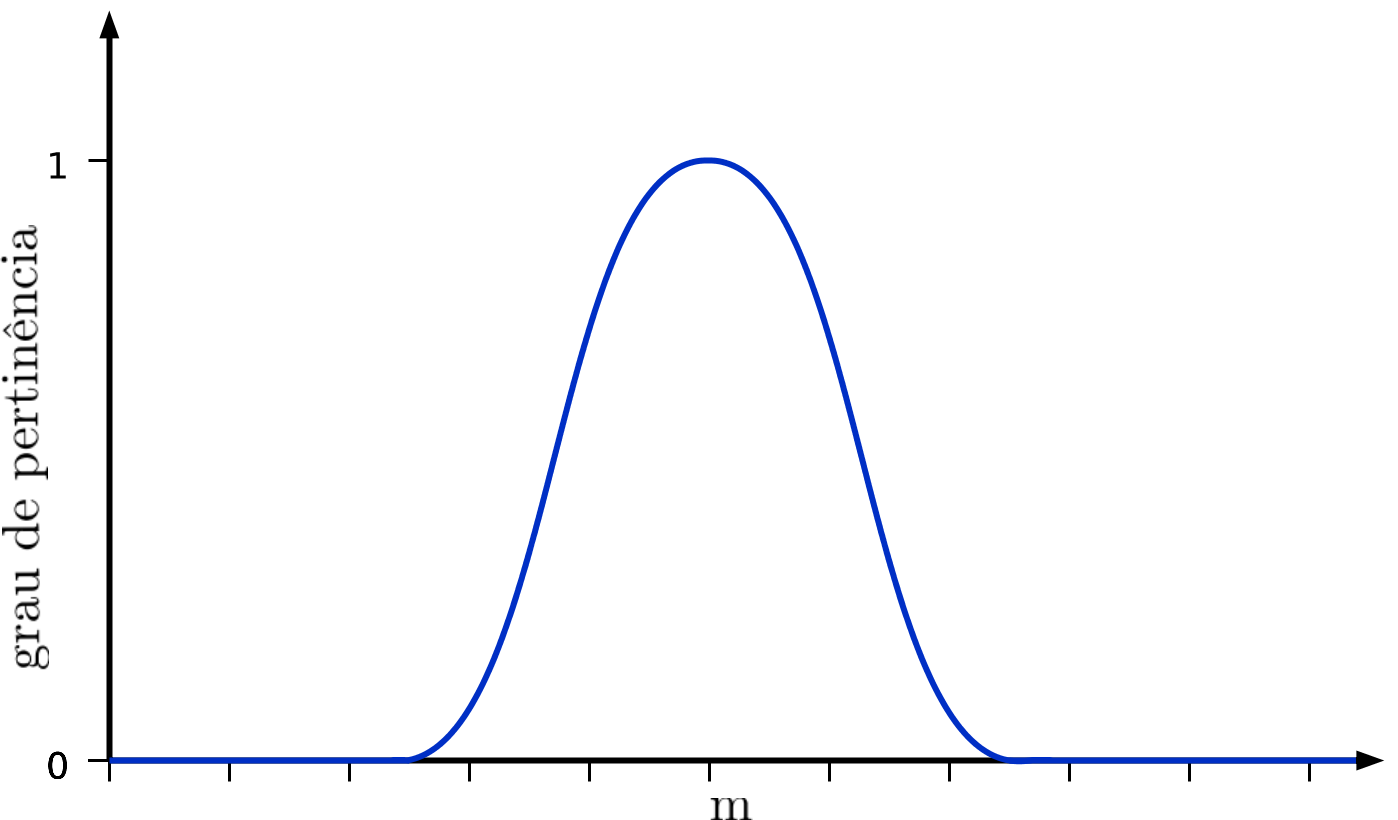
\includegraphics[width=1\textwidth]{funcao_gaussiana}
\end{figure}
\end{columns}
\end{frame}

%------------------------------------------------------
\subsection{Classificadores}
\begin{frame}{Introdução}
Seja o conjunto de dados de treinamento com $N$ amostras da forma:
\begin{equation*}
    D = (x_1, y_1), (x_2, y_2), \ldots, (x_N, y_N)
\end{equation*}
\noindent onde $i = 1, 2, \ldots, N$, $y_i \in Y$ e $Y = \{+1, -1\}$, e cada $x_i$ é um vetor $d$-dimensional da forma:

\begin{equation*}
  x = 
  \begin{bmatrix}
    a_1 \\ a_2 \\ \vdots \\ a_d
  \end{bmatrix}
\end{equation*}
\noindent onde $x \in X$ e $X$ é o espaço de entrada, ou seja, todos os $x$ vetores possíveis.
\end{frame}

%------------------------------------------------------
\begin{frame}{Máquinas de Vetores Suporte (SVM)}
\begin{columns}
\column{0.45\textwidth}
\begin{itemize}
    \item SVMs têm a habilidade de gerar um hiperplano ou conjunto de hiperplanos num espaço de alta ou infinita dimensionalidade \citep{duda:12}
    \item Assumindo que $D$ é linearmente separável \citep{lorena:03}
\end{itemize}

\column{0.55\textwidth}
\begin{figure}[!h]
  \centering
  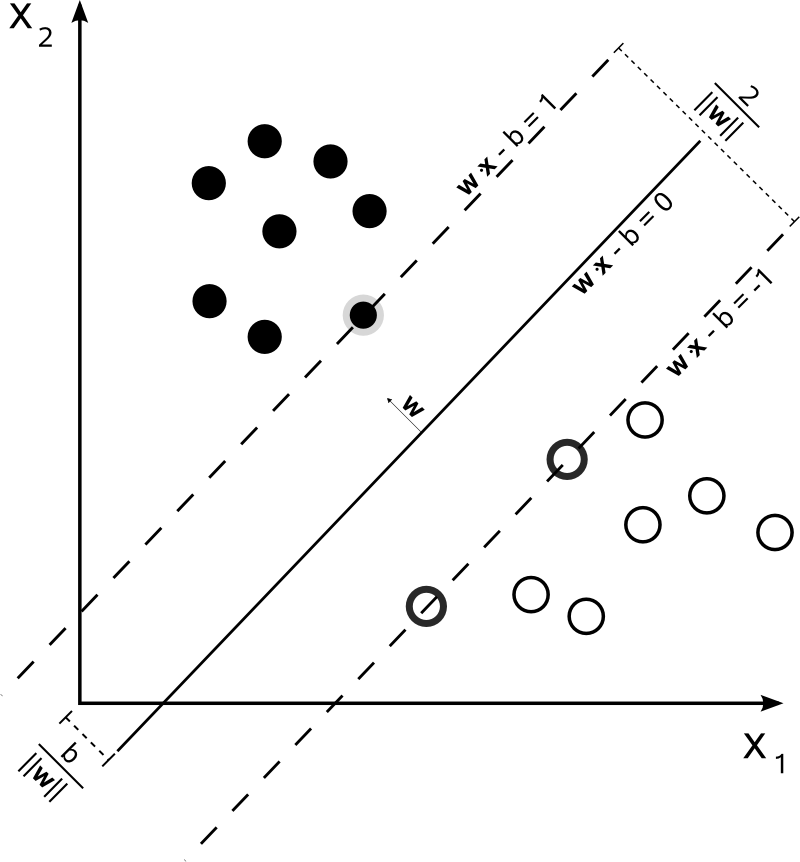
\includegraphics[width=1\textwidth]{svm_max_sep_hyperplane_with_margin}
\end{figure}
\end{columns}

\end{frame}

%------------------------------------------------------
\begin{frame}{Máquinas de Vetores Suporte (SVM)}
\begin{itemize}
    \item A minimização de $||w||$ maximiza a margem e, sendo assim, tem-se um problema de otimização
    \item $w$ e $b$ ótimos que resolvem este problema definem o classificador e podem ser obtidos por multiplicadores de Lagrange \citep{campbell:00}:
\end{itemize}
\begin{equation*}
\text{Maximizar: } \sum_{i=1}^N \alpha_i - \frac{1}{2} \sum_{i, j=1}^N \alpha_i \alpha_j y_i y_j x_i\cdot x_j
\end{equation*}

\begin{equation*}
\text{Sujeito a: }
\begin{cases}
    0 \leq \alpha_i \leq C\\[1em]
    \sum_{i=1}^N \alpha_i y_i = 0
\end{cases}
\end{equation*}

\end{frame}

%------------------------------------------------------
\begin{frame}{Máquinas de Vetores Suporte (SVM)}
SVMs lineares podem ser estendidas:
\begin{equation*}
    D' = (\Phi(x_1), y_1), (\Phi(x_2), y_2), \ldots, (\Phi(x_N), y_N)
\end{equation*}

A forma do hiperplano ótimo agora é definida por:
\begin{equation*}
w \cdot \Phi(x) + b = 0
\end{equation*}

O problema de otimização pode ser resolvido como \citep{lorena:03}:
\begin{equation*}
\text{Maximizar: } \sum_{i=1}^N \alpha_i - \frac{1}{2} \sum_{i, j=1}^N \alpha_i \alpha_j y_i y_j \Phi(x_i)\cdot \Phi(x_j)
\end{equation*}

\end{frame}

%------------------------------------------------------
\begin{frame}{Máquinas de Vetores Suporte (SVM)}
\emph{Kernels} são funções que têm a finalidade de projetar os vetores de entrada num espaço de características com número de dimensões exponencial ou infinito \citep{taylor:04}:
\begin{equation*}
k(x_i, x_j) =  \Phi(x_i) \cdot \Phi(x_j)
\end{equation*}

Alguns dos \emph{kernels} mais utilizados são \citep{lorena:03}:
\begin{itemize}
\item \emph{Kernel} linear
\begin{equation*}
k(x_i, x_j) =  (x_i \cdot x_j)
\end{equation*}

\item \emph{Kernel} polinomial
\begin{equation*}
k(x_i, x_j) =  ({\gamma x_i \cdot x_j + r} )^g
\end{equation*}

\item \emph{Kernel} gaussiano ou RBF
\begin{equation*}
k(x_i, x_j) =  \exp{\big(-\gamma {||x_i - x_j||}^2 \big)}
\end{equation*}
\end{itemize}

\end{frame}

%------------------------------------------------------
\begin{frame}{$k$-Vizinhos Mais Próximos ($k$-NN)}
\begin{columns}
\column{0.35\textwidth}
\begin{itemize}
    \item $k$-NN é um algoritmo baseado em instâncias
    \item Rotula uma nova amostra $x$ com a classe de maior frequência dentre as $k$ mais próximas
    \item Decisão por maioria de votos \citep{duda:12}
\end{itemize}

\column{0.65\textwidth}
\begin{figure}[!h]
  \centering
  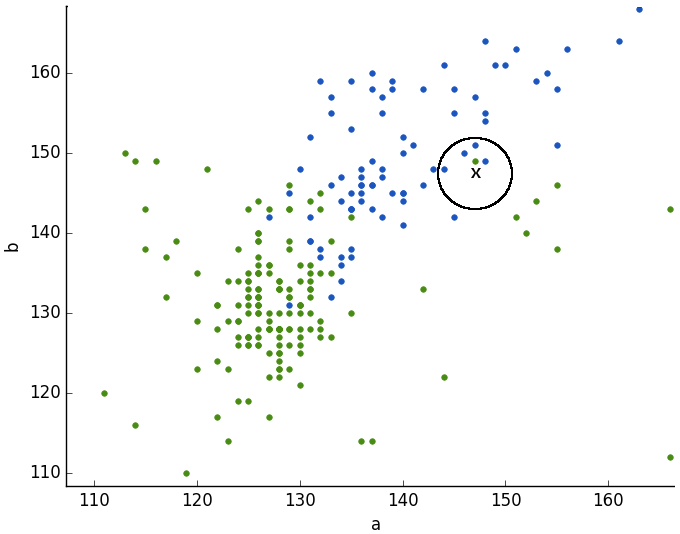
\includegraphics[width=1\textwidth]{knn_exemplo}
\end{figure}
\end{columns}

\end{frame}

%------------------------------------------------------
\begin{frame}{$k$-Vizinhos Mais Próximos ($k$-NN)}
A distância entre duas amostras $x_i$ e $x_j$ quaisquer pode ser obtida em termos da distância Euclidiana:
\begin{equation*}
\label{eq:knn_distancia_euclidiana}
d(x_i, x_j) = \sqrt{\sum_{r=1}^d (a_r(x_i) - a_r(x_j))^2}
\end{equation*}

Para classificar uma nova amostra $x_q$ \citep{mitchell:97}:
\begin{equation*}
\label{eq:knn_funcao_argmax}
g(x_q) \gets \argmax_{y \in Y} \sum_{i=1}^k \delta (y, f(x_i))
\end{equation*}
\noindent onde
\begin{equation*}
\label{eq:knn_delta}
  \delta (y, f(x_i)) =  \begin{cases}
                1, \quad \text{se}\ y = f(x_i) \\
                0, \quad \text{caso contrário}
              \end{cases}
\end{equation*}
\end{frame}

%------------------------------------------------------
\begin{frame}{$k$-Vizinhos Mais Próximos ($k$-NN)}
\begin{itemize}
    \item Uma variação da função é a atribuição de pesos a cada um dos $k$ vizinhos, conforme sua distância
    \item Implica que pontos mais próximos de $x_q$ têm maior influência na sua rotulação
\end{itemize}
\begin{equation*}
g(x_q) \gets \argmax_{y \in Y} \sum_{i=1}^k w_i \delta (y, f(x_i))
\end{equation*}
\noindent onde
\begin{equation*}
  w_i = \frac{1}{d(x_q, x_i)^2}
\end{equation*}

\end{frame}

%------------------------------------------------------
\begin{frame}{Árvores de decisão}
\begin{itemize}
    \item Processo iterativo onde um atributo (nó) é escolhido como raiz até algum nó folha, onde a classe é atribuída à amostra
    \item ID3 avalia cada atributo através de um teste estatístico para determinar o quão bem ele, por si só, classifica as amostras de treinamento \citep{quinlan:86}
    \item Um ramo descendente do nó raiz é criado para cada valor possível deste atributo \citep{mitchell:97}
    \item C4.5 estende o ID3 para possibilitar o uso de atributos contínuos, dados ausentes e poda da árvore \citet{quinlan:93}
\end{itemize}
\end{frame}

%------------------------------------------------------
\begin{frame}{Árvores de decisão}
Para medir a impureza de uma partição, o ID3 usa o conceito de entropia \citep{quinlan:86}:

\begin{equation*}
H(D) = - y_\oplus log_2 y_\oplus - y_\ominus log_2 y_\ominus
\end{equation*}

O teste estatístico, conhecido como ganho de informação, mede a efetividade de um atributo na classificação dos dados \citep{quinlan:86}:
\begin{equation*}
IG(D, a_r) = H(D) - \sum_{v \in V(a_r)} \frac{|D_v|}{|D|} H(D_v)
\end{equation*}

\end{frame}